\documentclass[a4paper]{article}
\usepackage[utf8]{inputenc}
\usepackage[russian,english]{babel}
\usepackage[T2A]{fontenc}
\usepackage[left=10mm, top=20mm, right=18mm, bottom=15mm, footskip=10mm]{geometry}
\usepackage{indentfirst}
\usepackage{amsmath,amssymb}
\usepackage[italicdiff]{physics}
\usepackage{graphicx}
\graphicspath{{images/}}
\DeclareGraphicsExtensions{.pdf,.png,.jpg}
\usepackage{wrapfig}
\usepackage{pgfplots}

\usepackage{caption}
\captionsetup[figure]{name=Рисунок}
\captionsetup[table]{name=Таблица}


\title{\underline{Лабораторной работы 1.2.3}}
\author{Старостин Александр, Б01-401}
\date {12 Октября, 2024 год}


\begin{document}

\maketitle
\newpage

\textbf{Определение моментов инерции твердых тел с помощью трифилярного подвеса}

\section{Аннотация}
    \par \textbf{Цель работы:} измерение момента инерции тел и сравнение результатов с расчетми по теоретиеским формулам; проверка аддитивноски моментов инерции и справедливости формулы Гюйгенса-Штейнера.\\

    \par \textbf{В работе используются:} трифилярный подвес, секундомер, счетчик числа колебаний, набор тел, момент инерции которых надлежит измерить (диск, стержень, полный цилиндр и другие).

\section{Теоретические сведения}

\par Инерционность при вращении тела относительно оси определяется моментом инерции тела относительно этой оси. Момент инерции твердого тела относительно неподвижной оси вращения вычисляется по формуле:

\begin{equation}
	I = \int r^2 dm
\end{equation}

где $r$ - расстояние от оси вращения до любой материальной точки тела $dm$ - масса люой материальной точки.\\

Для тел сложной формулы можно посчитать момент инерции с помощью трифилярного подвеса:

\begin{figure}[!ht]
    \centering
    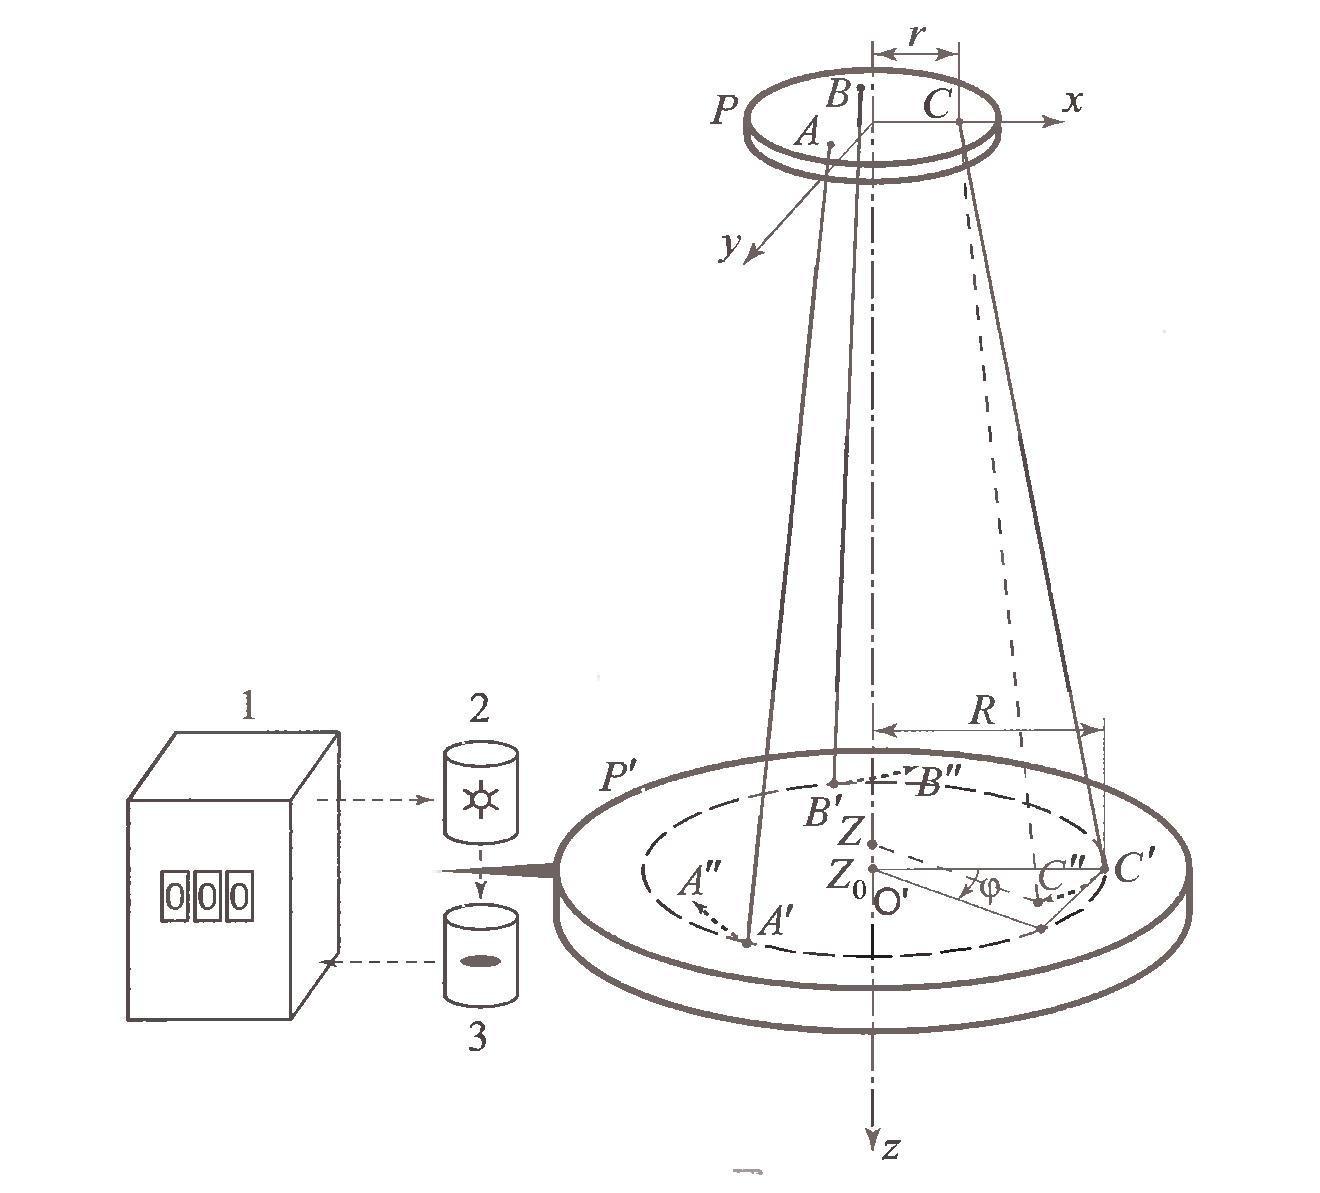
\includegraphics[scale=0.3]{podves.jpg}
    \caption{Трифилярный подвес}
\end{figure}

\newpage

С помощью него создаются крутильные колебния. Если считать их незатухающими, то из решения уравнения колебания получаем для системы - тело и подвижная платформа:

\begin{equation}
	{T} = {2\pi}\sqrt{\frac{Iz_0}{mgRr}}
\end{equation}

и

\begin{equation}
	{I} = \frac{mgRrT{^2}}{4\pi{^2}z_0}
\end{equation}

где $I$ - момент инерции системы, $m$ - суммарная масса системы, $R$ - радиус подвижной платформы, $r$ - радиус неподвижной платформы, $T$ - период вращательных колебаний, $z_0$ - Расстояние между центрами платформ до начала колебаний.\\

Тк для одного и того же подвеса $R$, $r$ и $z_0$ постоянные, то:

\begin{equation}
	{I} = {kmT{^2}}
\end{equation}

\item где $k$ = $\frac{gRr}{4\pi{^2}z_0}$ = $const$\\

Таким образом, момент инерции тела будет равен разности момента инерции системы и момента инерции подвижной платформы.\\



В ходе работы нужно будет проверить закон аддитивности для моментов инерции и теорему Гюгенса-Штейнера.\\

Закон аддитивности:\\
Момент инерции сложного тела равен сумме моментов инерции всех частей тела, из которых оно состоит.
Чтобы это проверить, посчитаем моменты инерции для кастрюли, крышки и их соединения. Сравнив сумму первых двух с третьем, увидим, что закон аддитивности верен.\\

Теорема Гюгенса-Штейнера:\\
Момент инерции относительно произвольной оси равен сумме момента инерции относительно оси, параллельной данной и проходящей через центр тела, и произведение массы тела на квадрат расстояния между ними.

\begin{equation}
	{I} = {I_0} + m * a^2
\end{equation}

Из формул (3) и (4) получаем, что $T^2$ линейно зависит от $a^2$. Проверив это, мы сможем доказать справедливость теоремы Гюгенса-Штейнера.\\

\section{Ход работы}

\subsection{Проверка установки.}

Измерения проходят для ненагруженной платформы.\\

При возбуждении крутильных колебаний устройство функционирует нормально. Нежелательные маятниковообразные движения платформы не возникают. Счётчик числа колебаний работает нормально.
Значит, на данной установке можно проводить работу.\\


\subsection {Проверка того, что колебания можно считать незатухающими.}

    Измерения проходят для ненагруженной платформы.\\

    Измерим амплитуду колебаний в начале колебаний и через 30 периодов:

    \begin{table}[h!]
    \begin{center}
    \begin{tabular}{|c|c|}
    \hline
    Количество прошедших колебаний $N$    & $\varphi$, \circ   \\ \hline

    1    & 35         \\ \hline
    30   & 30       \\ \hline

    \end{tabular}
    \caption{Таблица измерений ампилитуды колебаний}
    \end{center}
    \end{table}

    Спустя 30 колебаний ампилитуда колебаний изменилась в $\frac{30}{35}$ = 0,86 раза. Тк амплитуда за 30 колебаний уменьшается меньше, чем в два раза (0,86 < 2), то колебания можно считать не затухающими.


\subsection {Проверка того, что при разных амплитудах периоды крутильных колебаний одинаковые.}

    \begin{table}[h!]
    \begin{center}
    \begin{tabular}{|c|c|c|c|}
    \hline
    $\varphi$, \circ    & Время $t$, с    & Количество колебаний $N$    & Период $T$, с   \\ \hline

    20   & 87,44   & 20  & 4,37      \\ \hline
    30   & 88,33   & 20  & 4,42      \\ \hline

    \end{tabular}
    \caption{Таблица измерений периодов при разных ампилитудах }
    \end{center}
    \end{table}

    Все периоды можно считать равными. Значит, при разных амплитудах периоды колебаний одинаковые и, следовательно, период колебаний не зависит от начальной амплитуды.

\subsection {Параметры установки.}

\item Длина любой проволки: $l = 124,4 \pm{0,1}$ см.
\item Расстояние от центра диска до любой из точек крепления проволок к диску $R_0 = 10,4 \pm{0,1}$ см.\\
\item Диаметр нижнего диска: $d = 2R = 24,8 \pm{0,2}$ см.
\item Радиус нижнего диска: $R = 12,4 \pm{0,1}$ см.\\
\item Радиус верхнего диска: $r = 3,02 \pm{0,03}$ см.\\
\item Вертикальное расстояние: $z_0 = \sqrt{l^2 - R_0^2} = 124,0 \pm{0,1}$ см.\\

\item Коэффициент $k$: $k = \frac{gR_0r}{4\pi{^2}z_0} = 6,29$ см$^2$/c$^2$ $= 6,29 * 10^{-4}$ м$^2$/c$^2$
\item Погрешность коэффициента: $\sigma_{k} = k * \sqrt{(\frac{\sigma_{R_0}}{R_0})^2 + (\frac{\sigma_{z_0}}{z_0})^2 + (\frac{\sigma_{r}}{r})^2}$ = 0,09 * 10$^{-4}$ м$^2$/c$^2$.\\

\item Тогда $k = (6,29 \pm{0,09}) * 10^{-4}$ м$^2$/c$^2$.\\

\subsection {Момент инерции платформы.}

\item Масса платформы: $m_0 = 1066,0 \pm{0,3}$ г.
\item Период для платформы: $T_0 = 4,39 \pm{0,03}$ с.\\
\item По формуле (4) момент инерции платформы: $I_0 = 0,0129$ кг * м$^{2}$.
\item Погрешность момента инерции платформы: $\sigma_{I_0} = I_0 * \sqrt{(\frac{\sigma_{k}}{k})^2 + (\frac{\sigma_{m}}{m})^2 + 4 * (\frac{\sigma_{T}}{T})^2}$ = 0,0003 кг * м$^{2}$.
\item Тогда момент инерции плаформы: $I_0 = 0,0129 \pm{0,0003}$ кг * м$^{2}$.\\

\subsection {Измерение моментов инерции тел, проверка закона аддетивности, теоретическое вычисление моментов инерции тел.}

Измерение моментов инерции тел:
\begin{table}[h!]
    \begin{center}
    \begin{tabular}{|c|c|c|c|}
    \hline

    тело    & масса тела $m$, г   & Период для тела с платформой $T$, с    & Момент инерции тела и платформы, кг * м$^{2}$     \\\hline

    Крышка     & 580,3 \pm{0,3}     & 3,94 \pm{0,03}   & 0,0161 \pm{0,0003}         \\ \hline
    Кастрюля   & 734,4 \pm{0,3}     & 4,24 \pm{0,03}   & 0,0204 \pm{0,0003}         \\ \hline
    Вместе    & 1314,7 \pm{0,3}     & 3,98 \pm{0,03}   & 0,0237 \pm{0,0003}         \\ \hline

    \end{tabular}
    \caption{Таблица измерений ампилитуды колебаний}
    \end{center}
    \end{table}

    \item Момент инерции крышки:    $I_1 = 0,0161 - 0,0129 = 0,0032$ кг * м$^{2}$.
    \item Погрешность момента инерции крышки: $\sigma_{I_1} = I_1 * \sqrt{\sigma_{I_0}^2 + \sigma_{I_{10}}^2}$ = 0,0004 кг * м$^{2}$.
    \item Тогда момент инерции крышки: $I_1 = 0,0032 \pm{0,0004}$ кг * м$^{2}$.\\

    \item Момент инерции кастрюли:  $I_2 = 0,0204 - 0,0129 = 0,0075$ кг * м$^{2}$.
    \item Погрешность момента инерции кастрюли: $\sigma_{I_2} = I_2 * \sqrt{\sigma_{I_0}^2 + \sigma_{I_{20}}^2}$ = 0,0004 кг * м$^{2}$.
    \item Тогда момент инерции кастрюли: $I_2 = 0,0075 \pm{0,0004}$ кг * м$^{2}$.\\

    \item Момент инерции суммарный: $I_3 = 0,0237 - 0,0129 = 0,0108$ кг * м$^{2}$.
    \item Погрешность суммарного момента инерции: $\sigma_{I_3} = I_3 * \sqrt{\sigma_{I_0}^2 + \sigma_{I_{30}}^2}$ = 0,0004 кг * м$^{2}$.
    \item Тогда суммарный момент инерции: $I_3 = 0,0108 \pm{0,0004}$ кг * м$^{2}$.\\

    \item $I_1 + I_2 = 0,0107 \approx 0,0108 = I_3$. Значит закон аддетивности верен.\\

    Теоретические вычисления моментов инерции тел:\\

    Из формулы (1) момент инерции сплошного однородного цилиндра: $I = \frac{1}{2} * m * R^2 = \frac{1}{8} * m * d^2$
    Из формулы (1) момент инерции полового однородного цилиндра: $I = \frac{1}{2} * m * (R^2 + r^2) = \frac{1}{8} * m * (D^2 + d^2)$\\
    Для крышки:\\
    Размеры: диаметр ручки = 1,00 см; высота ручки = 2,90 см; диаметр диска = 17,05 см; высота ручки = 0,35 см. (Погрешность составляет 0,01 см).
    Теоретический $I_1 = 0,0030 \pm{0,0003}$ кг * м$^{2}$.\\

    Для кастрюли:\\
    Размеры: диаметр внешний = 16,7 см; высота = 4,06 см; диаметр внутренний = 14,73 см; высота ручки = 0,35 см. (Погрешность составляет 0,01 см).
    Теоретический $I_2 = 0,0064 \pm{0,0003}$ кг * м$^{2}$.\\

    Теоретические расчёты приблизительно совпали с результатами измерений. Значит, метод измерения моментов инерции тел верен.\\

\subsection {Проверка теоремы Гюгенса-Штейнера.}

Из теоретической части следует, что теореа верна если $T^2$ линейно зависит от $a^2$.\\

Возьмём диск, разрезанный по диаметру. Вычислим для него пероиды для каждого смещения его частей вдоль диска и посторим график зависимости $T^2$ от $a^2$:

    \begin{table}[h!]
    \begin{center}
    \begin{tabular}{|c|c|c|c|c|}
    \hline

    Расст. между центрами полудисков $a$, см   & Время $t_1$, с  & Время $t_2$, с  & Колчество колебаний $N$ & Средний период $T$, с     \\\hline

    0.0     & 31,26      & 31,16    & 10   & 3,12          \\ \hline
    1.0     & 31,29      & 31,22    & 10   & 3,13          \\ \hline
    2.0     & 31,39      & 31,42    & 10   & 3,14          \\ \hline
    3.0     & 31,76      & 31,67    & 10   & 3,17          \\ \hline
    4.0     & 32,18      & 32,06    & 10   & 3,21          \\ \hline
    5.0     & 32,49      & 32,56    & 10   & 3,25          \\ \hline
    6.0     & 33,37      & 33,28    & 10   & 3,33          \\ \hline
    7.0     & 33,79      & 33,93    & 10   & 3,37          \\ \hline
    8.0     & 34,72      & 34,63    & 10   & 3,47          \\ \hline
    9.0     & 35,56      & 35,58    & 10   & 3,56          \\ \hline
    10.0     & 36,5      & 36,49    & 10   & 3,65          \\ \hline
    11.0     & 37,52      & 37,56    & 10   & 3,75          \\ \hline
    12.0     & 38,42      & 38,50    & 10   & 3,85          \\ \hline
    13.0     & 39,69      & 39,81    & 10   & 3,98          \\ \hline
    14.0     & 40,96      & 41,01    & 10   & 4,10          \\ \hline
    15.0     & 42,10      & 42,23    & 10   & 4,22          \\ \hline


    \end{tabular}
    \caption{Таблица измерений периодов колебаний и расстояний между центрами дисков.}
    \end{center}
    \end{table}

    \newpage

    Посторим график зависимости $T^2$ от $a^2$.\\


    \begin{figure}[!ht]
    \centering
    \begin{tikzpicture} [hu!]
    \begin{axis}[
    legend pos = north west,
    title  = {Зависимость $T^2$ от $a^2$},
    width  = {360},
    height = {320},
    ylabel = {$T^2$, с$^2$},
    xlabel = {$a^2$, см $^2$},
    minor tick num = 4,
    xmin   = {0},
    ymin   = {8},
    xmax   = {240},
    ymax   = {19}
    ]

    \legend{
        Измерения,
        Наилучшая прямая
    };

    \addplot [blue, mark = *] coordinates{
    (0, 9.73) (1, 9.80) (4, 9.86) (9, 10.05) (16, 10.30) (25, 10.56) (36, 11.09) (49, 11.36) (64, 12.04) (81, 12.67) (100, 13.32) (121, 14.06) (144, 14.82) (169, 15.84) (196, 16.81) (225, 17.81)};

    \addplot[dashed, draw = red] coordinates{
    (0, 9.72) (1, 9.76) (4, 9.86) (9, 10.05) (16, 10.30) (25, 10.62) (36, 11.01) (49, 11.48) (64, 12.02) (81, 12.63) (100, 13.31) (121, 14.07) (144, 14.90) (169, 15.79) (196, 16.77) (225, 17.81)};

    \end{axis}
    \end{tikzpicture}
\end{figure}

    Расчёты по МНК:

    \item $c = \frac{\langle T^2 a^2 \rangle - \langle T^2 \rangle \langle a^2 \rangle}{\langle a^4 \rangle - (\langle a^2 \rangle)^2} = 0,035945$ c$^2$/см$^2$ $= 359,45$ c$^2$/м$^2$\\
    \item $b = \langle T^2 \rangle - c * \langle a^2 \rangle = 9,72$ c$^2$\\
    \item Наилучшая прямая: $T^2 = c * a^2 + b$\\

    Из графика видно, что $T^2$ действительно зависит линейно от $a^2$.\\

    Из формул (4) и (5) следует, что:

    \begin{equation}
	{T^2} = {\frac{I_0}{km}} + \frac{1}{k} a^2
    \end{equation}

    \item Из графика: $\frac{I_0}{km} = 9,72$ с$^2$.
    \item Масса диска $m = 1990,0 \pm{0,3}$ г.
    \item Из данных работы: $\frac{I_0}{km} = 10,31 \pm{0,28}$ с$^2$.\\

    Отношения приблизительно равны. Это говорит о справедливости теоремы Гюгенса-Штейнера.\\



\section{Вывод}

    Были измерены моменты инерции двух тел. Измерения моментов инерции совпали с теоритическими ожиданиями. Проверена верность закона аддетивности для моментов инерции тел и теоремы Гюгенса-Штейнера. Погрешность измерений приемлимая, что говорит о хорошей точности измерений.

\end{document}
